\chapter{Rysunki techniczne}
\begin{figure} [h]
\centering
%%----start of first subfigure----
	\subfloat[G�rna warstwa p�ytki]{\label{fig:subfig:front} 
	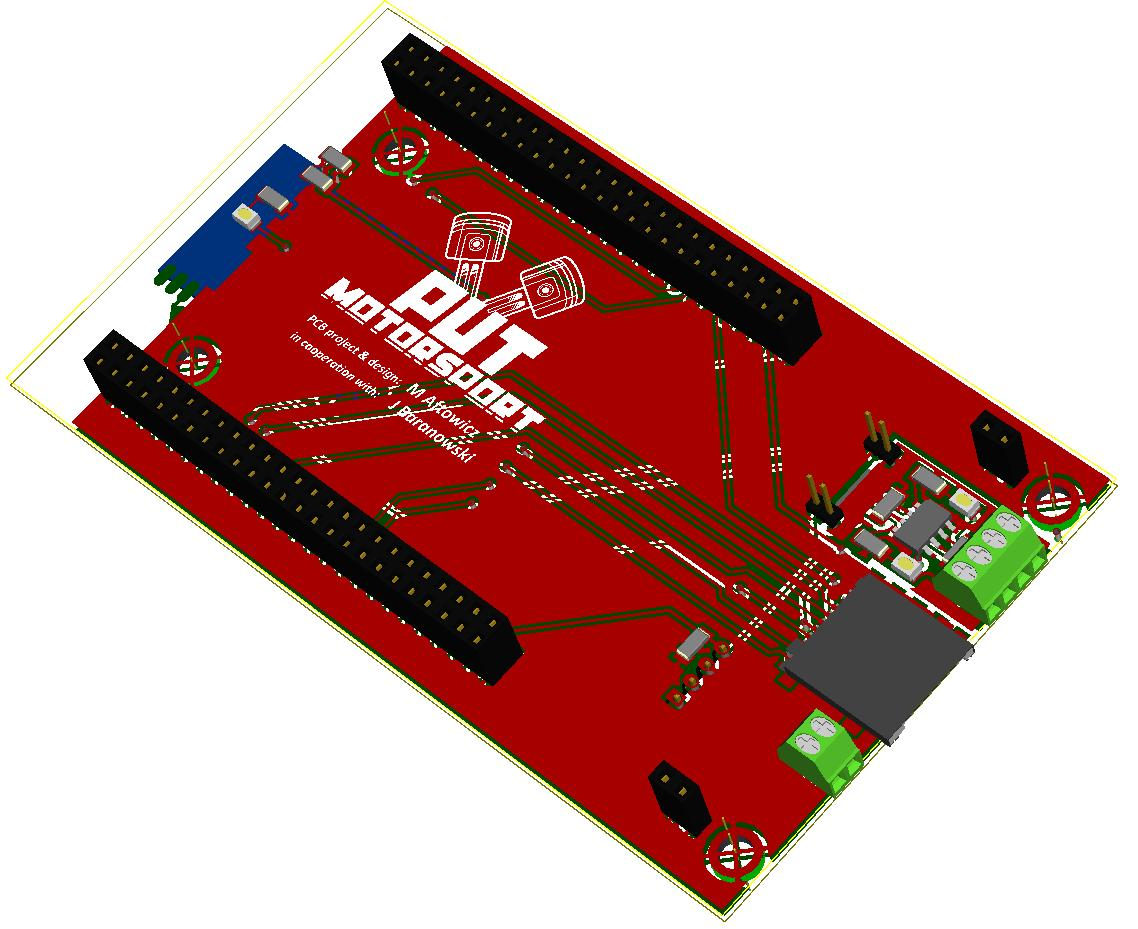
\includegraphics[height=0.3\textheight]{figures/Board_PCB_front.JPG}}
	\hfill
%%----start of second subfigure----
	\subfloat[Dolna warstwa p�ytki]{\label{fig:subfig:back}
	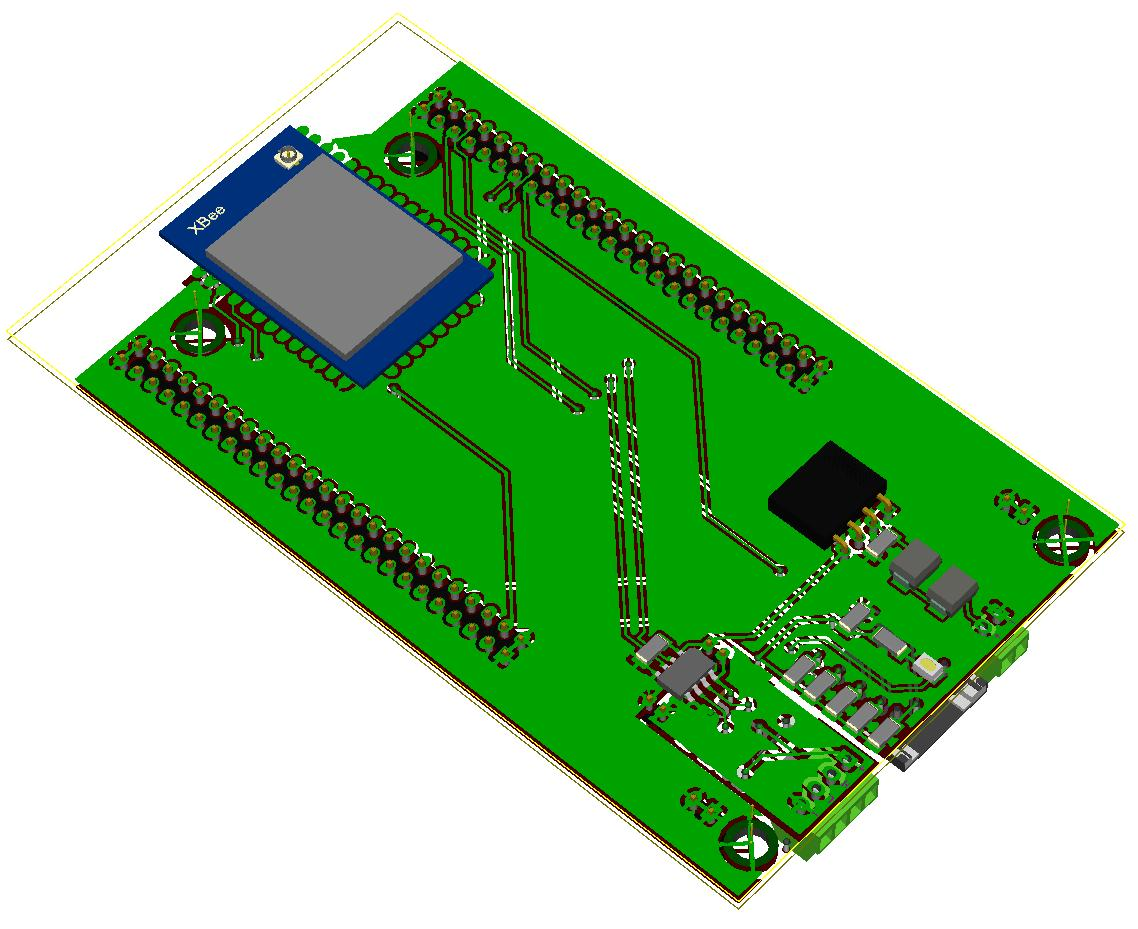
\includegraphics[height=0.3\textheight]{figures/Board_PCB_back.JPG}}
	\caption{Model 3D nak�adki na Discovery}
	\label{fig:3D} %% label for entire figure
\end{figure}

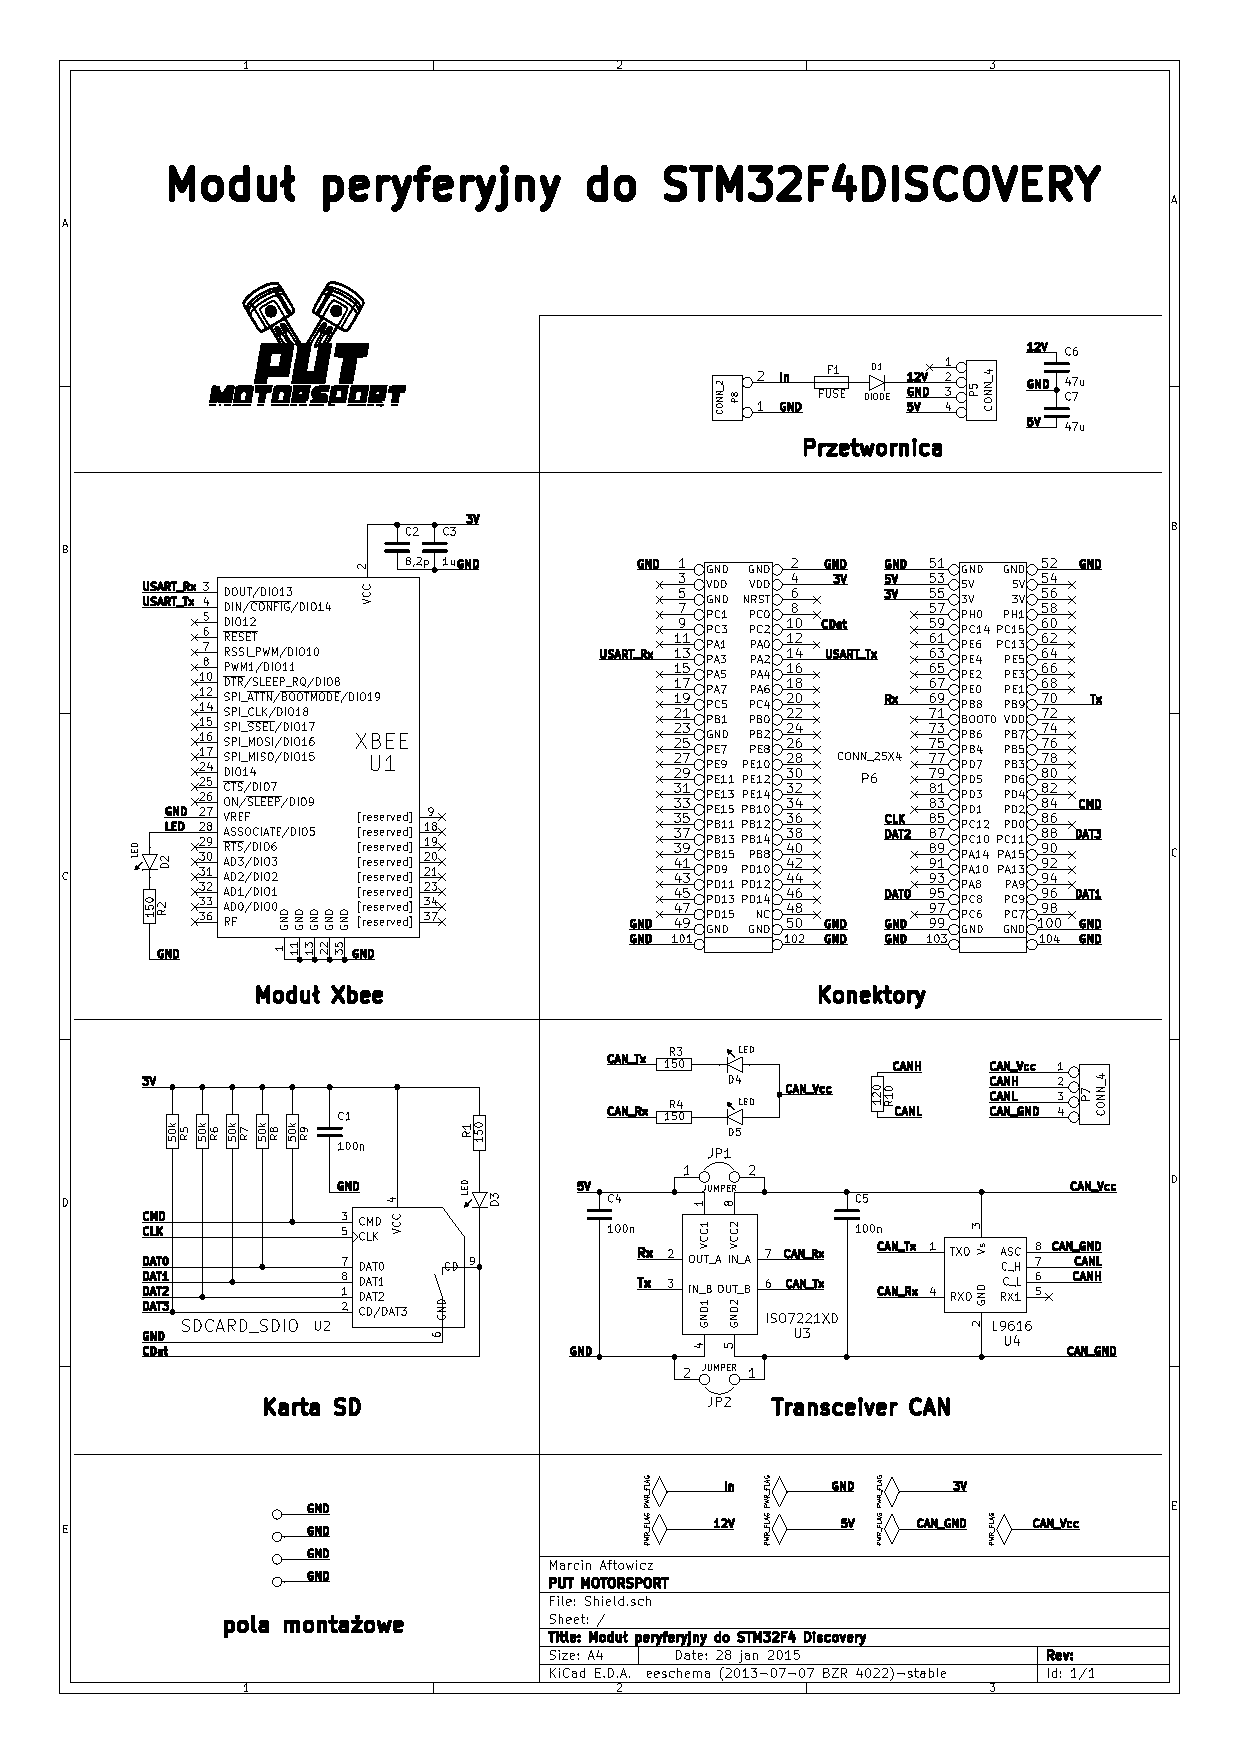
\includepdf[trim=0 0 -1cm 0, pages={1}]{figures/Motherboard_bw.pdf}
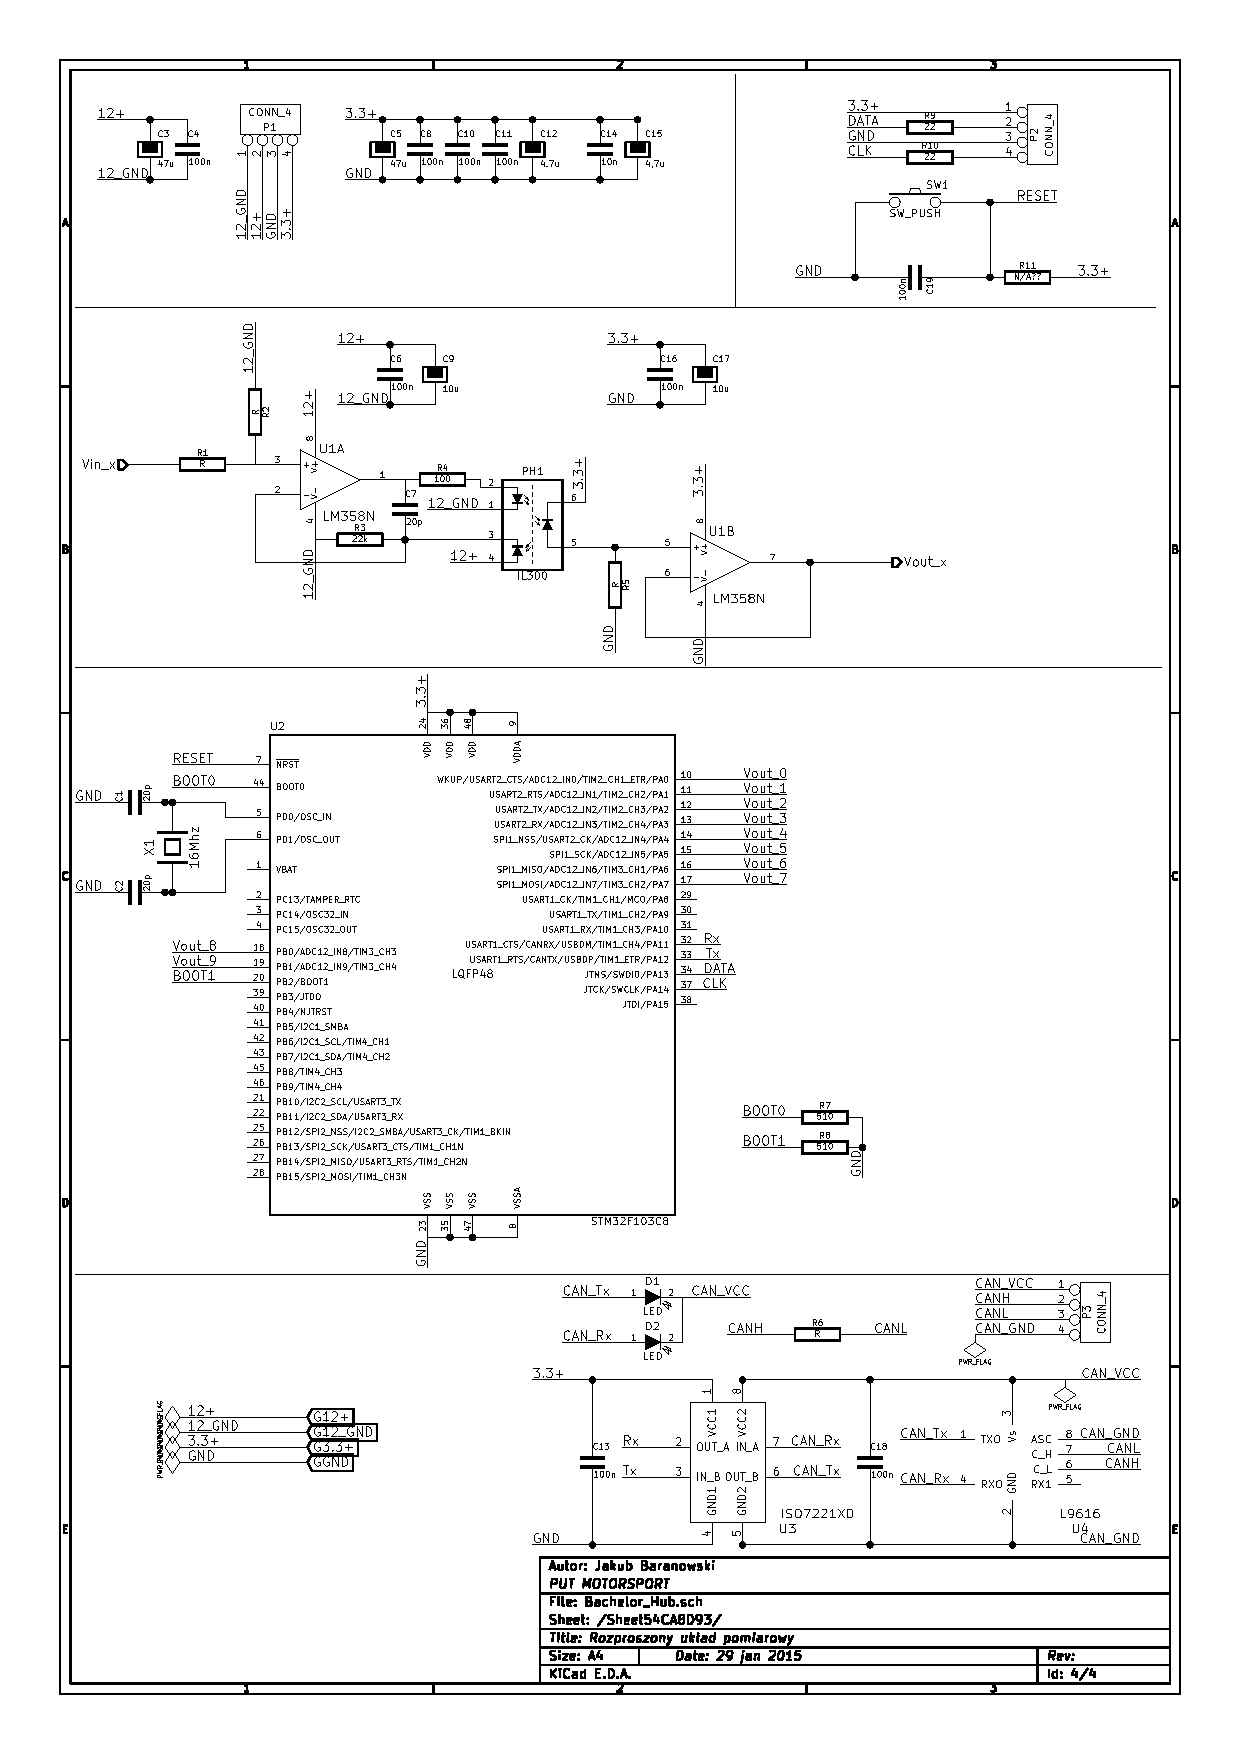
\includepdf[trim=-1cm 0 0 0, pages={1}]{figures/Bachelor_Hub.pdf}
\noindent


